
%(BEGIN_QUESTION)
% Copyright 2011, Tony R. Kuphaldt, released under the Creative Commons Attribution License (v 1.0)
% This means you may do almost anything with this work of mine, so long as you give me proper credit

Suppose the current through each of the ammeters is 2.81 amps, and the ratio of each current transformer is 100:5.  Calculate the horsepower output of this AC motor, assuming a power factor of 1 and an efficiency of 88\%:

$$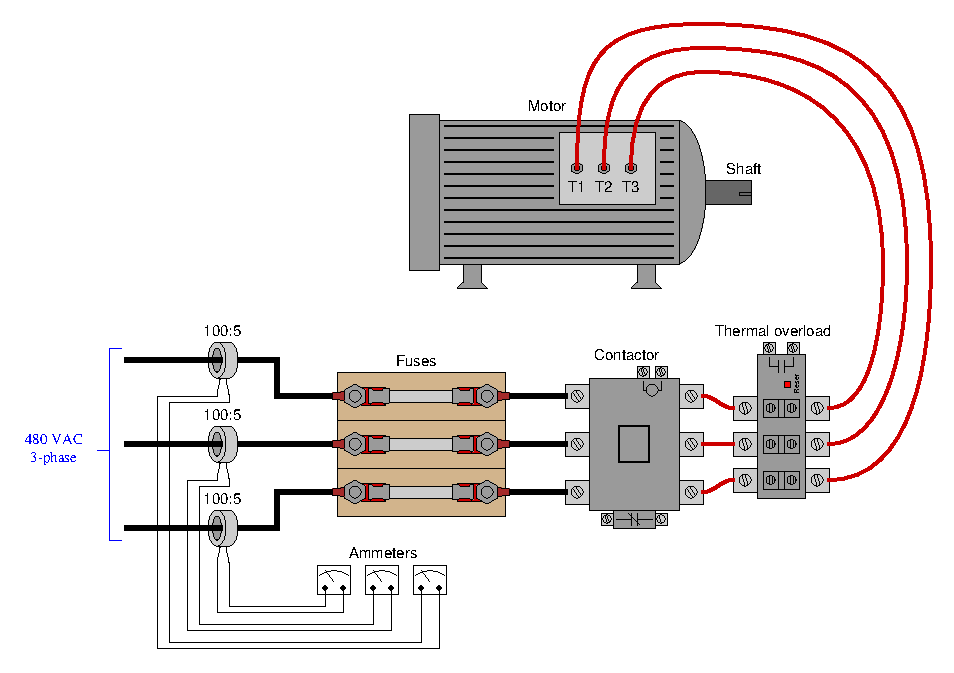
\includegraphics[width=15.5cm]{i01045x01.eps}$$

$P$ = \underbar{\hskip 50pt} horsepower

\vskip 10pt

\underbar{file i01045}
%(END_QUESTION)





%(BEGIN_ANSWER)

With 100:5 ratios at each CT, the line current to this motor is twenty times the amount of current through each ammeter:

$$(2.81) \left({100 \over 5}\right) = 56.2 \hbox{ amps}$$

At a line voltage of 480 VAC and a line current of 56.2 amps, the total electrical power in this 3-phase system may be calculated as follows:

$$P_{total} = (\sqrt{3}) (I_{line}) (V_{line})$$

$$P_{total} = (\sqrt{3}) (56.2) (480) = 46.724 \hbox{ kW}$$

At an efficiency of 88\%, only 88\% of this power becomes translated into mechanical horsepower.  This equates to 41.117 kW of mechanical power output at the motor shaft.

\vskip 10pt

Since we know there are 746 watts to every horsepower, we may convert this kW figure into HP as follows:

$$\left({41117 \hbox{ W} \over 1}\right) \left({1 \hbox{ HP} \over 746 \hbox{ W}}\right) = 55.12 \hbox{ HP}$$

%(END_ANSWER)





%(BEGIN_NOTES)


%INDEX% Electronics review: 3-phase electrical power 
%INDEX% Electronics review: current transformer (CT)

%(END_NOTES)


